\begin{frame}\frametitle{Long Baseline Neutrino Facility (LBNF) Experimental Setup}
\scriptsize
\begin{figure}
\label{fig:LBNF_overallScheme}
\centering
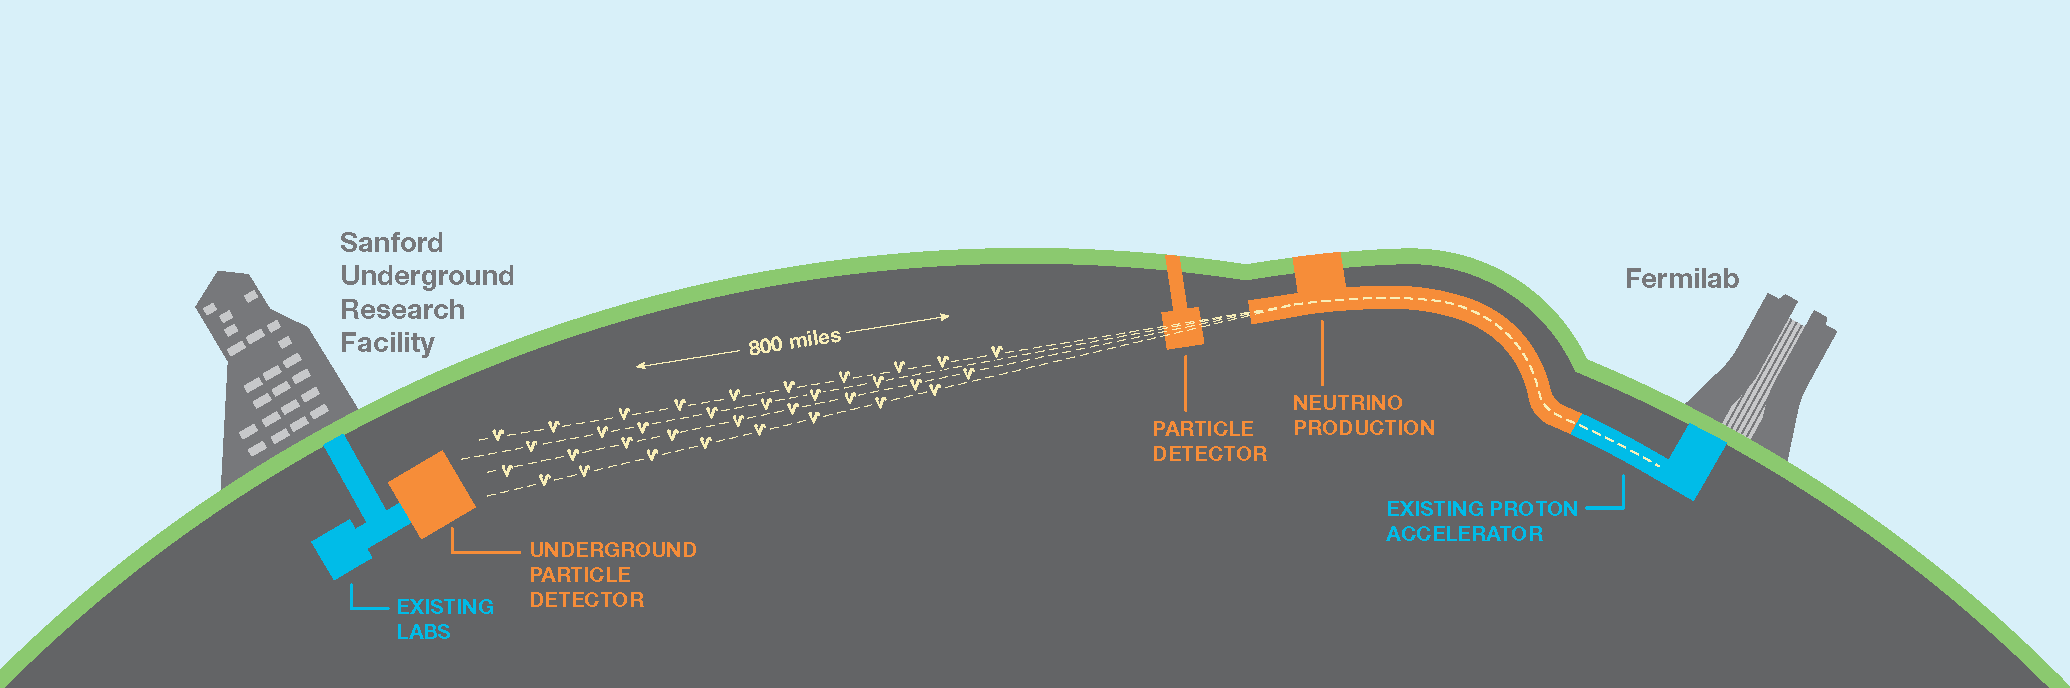
\includegraphics[width=0.95\textwidth, keepaspectratio=true]{figs/LBNF_overallScheme.png} 
\end{figure}
\begin{itemize}
  \item neutrino beam production system at FNAL, Illinois 
  \item near detector at FNAL, Illinois 
  \item far detector at SURF, South Dakota
\end{itemize}
\tiny
FNAL - Fermilab National Accelerator Laboratory, SURF - Sanford Underground Research Facility\\
Source of figure: \cite{ref_LBNFweb} 
\end{frame}

\begin{frame}
\begin{figure}
\label{fig:LBNF_FermilabAccComplex}
\centering
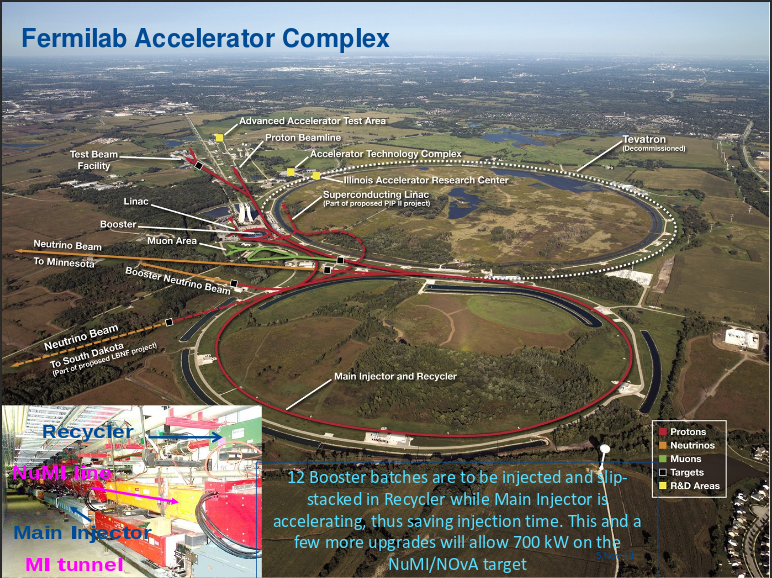
\includegraphics[width=0.95\textwidth, keepaspectratio=true]{figs/FermilabAccelerator.png}
\end{figure}
\end{frame}

\begin{frame}\frametitle{LBNF. Beam Production System}
\scriptsize
\begin{figure}
\label{fig:LBNF_nuBeam}
\centering
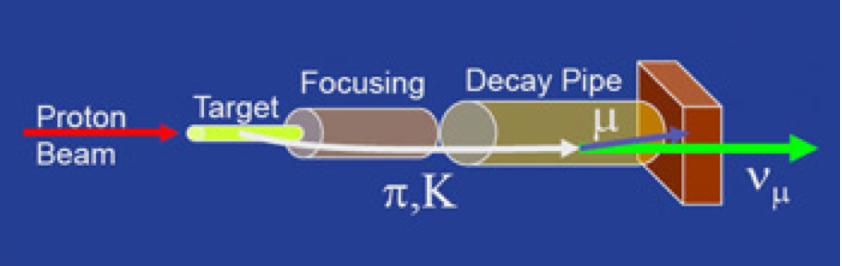
\includegraphics[width=0.45\textwidth, keepaspectratio=true]{figs/LBNF_nuBeam.png}  
\end{figure}
The neutrino beam production at the LBNF. Source of figure: \cite{ref_LBNFweb}\\
Pions (or kaons) are created: $p+p \rightarrow p+n+\pi^+$, $p+p \rightarrow p+\Delta^{++}+\pi^-$, $p+n \rightarrow p+p+\pi^-$, $p+n \rightarrow n+n+\pi^+$, $p+n \rightarrow p+\Delta^{-}+\pi^+$\\
And then decay: $\pi^+ \rightarrow \mu^+\nu_\mu$, $\pi^- \rightarrow \mu^-\bar{\nu_\mu}$, $K^+ \rightarrow \mu^+\nu_\mu$, $K^- \rightarrow \mu^-\bar{\nu_\mu}$\\
(Feynmann diagrams of these reactions are shown at the next slide)
\end{frame}

\begin{frame}\frametitle{LBNF. Pions and kaon creation and decay}
\scriptsize
\begin{figure}
\label{fig:pionAndKaonProductions}
\centering
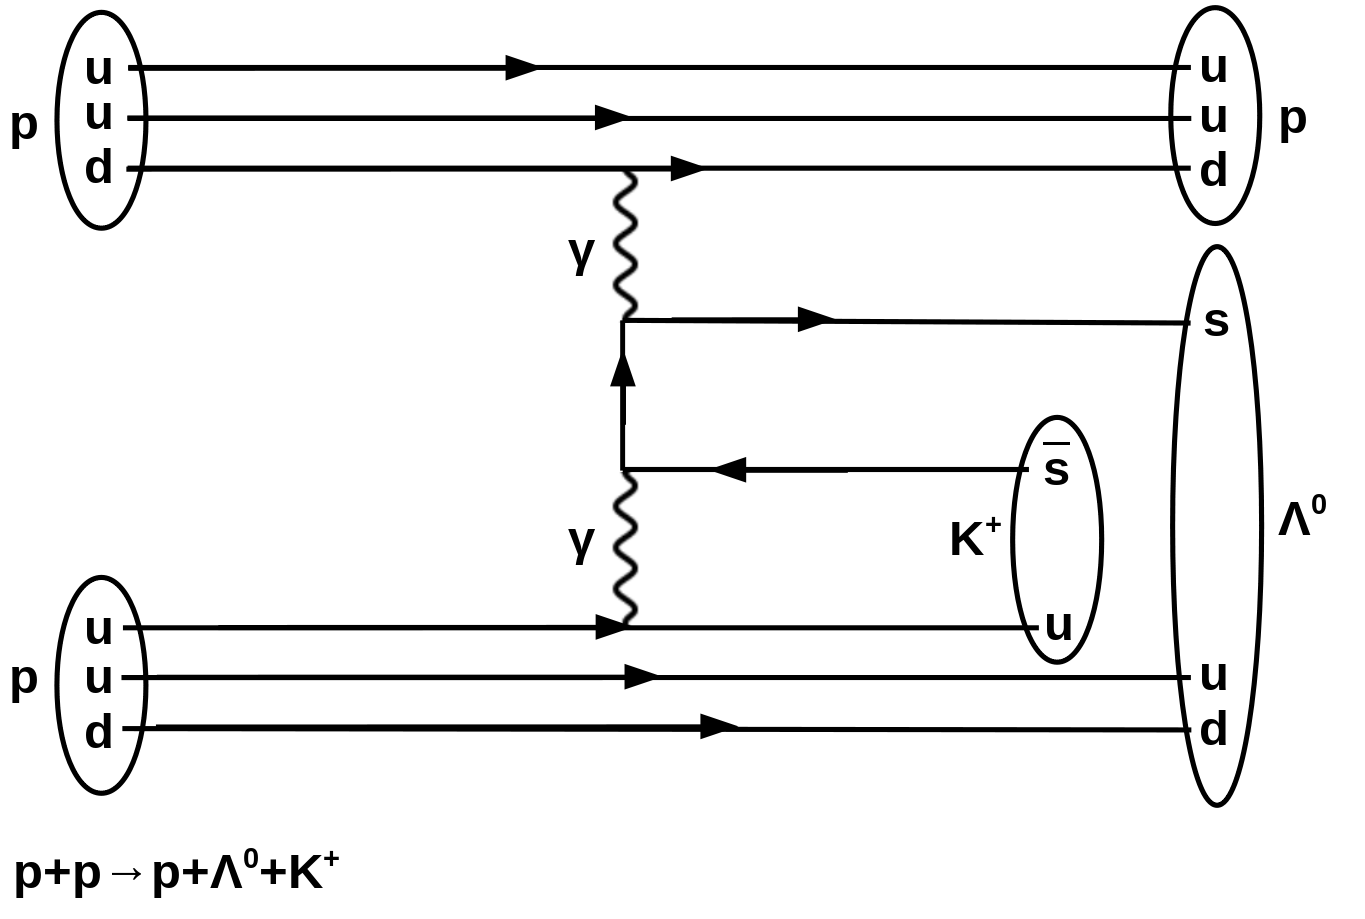
\includegraphics[width=0.48\textwidth, keepaspectratio=true]{figs/ppKaonProduction.png}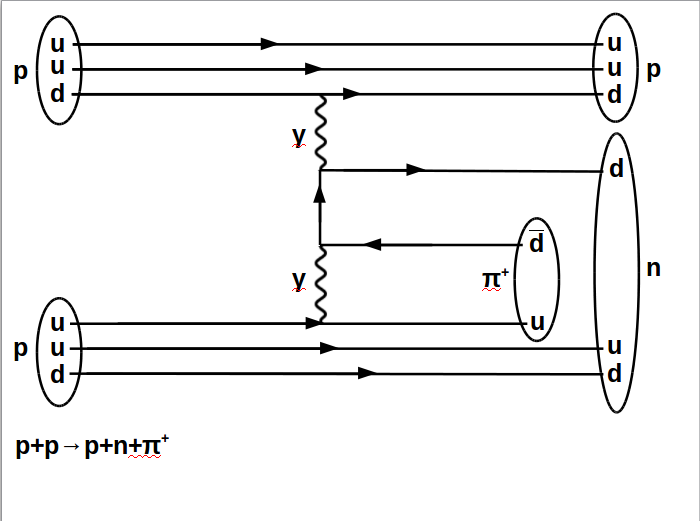
\includegraphics[width=0.48\textwidth, keepaspectratio=true]{figs/ppPionProduction.png}  
\end{figure}
\begin{figure}
\caption{Feynmann diagrams of charged pion and kaon decays to muon and muon antineutrino weakly through W-boson. Figures taken from \cite{ref_fig_pionandKaonDecays}.}
\label{fig:pionAndKaonDecays}
\centering
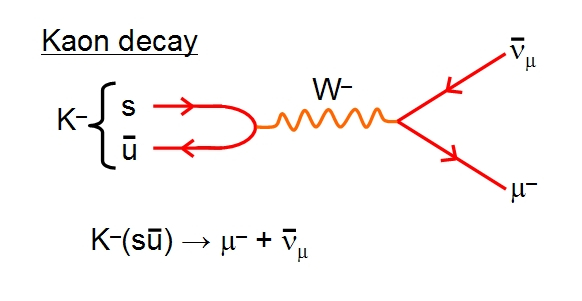
\includegraphics[width=0.45\textwidth, keepaspectratio=true]{figs/kaonDecay.jpg}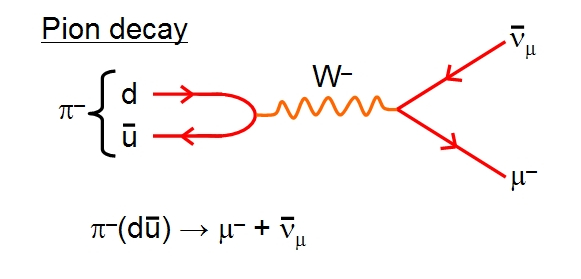
\includegraphics[width=0.45\textwidth, keepaspectratio=true]{figs/pionDecay.jpg} 
\end{figure}
\end{frame}

\begin{frame}\frametitle{LBNF. Near Detector}
\scriptsize
\begin{figure}
\label{fig:nearDetector}
\centering
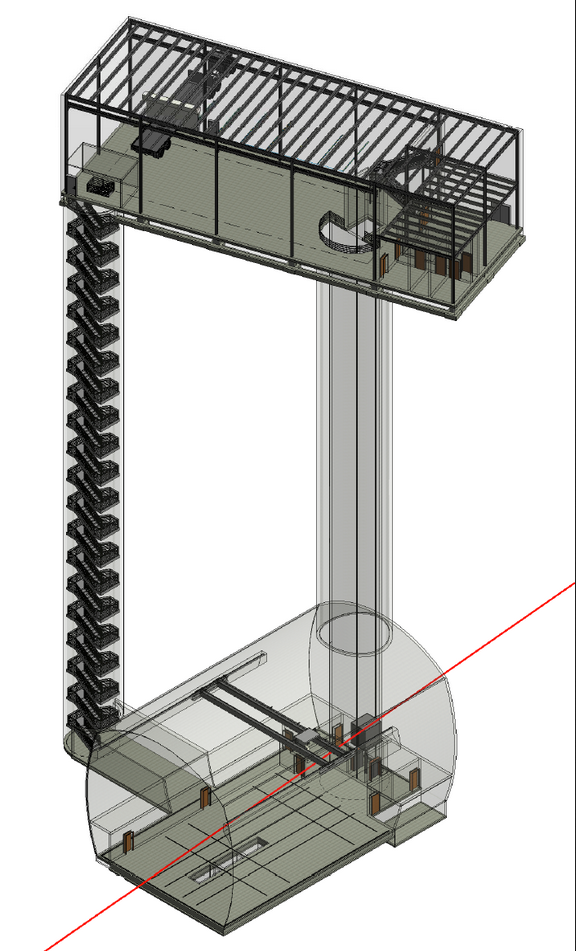
\includegraphics[width=0.25\textwidth, keepaspectratio=true]{figs/nearDetector_project.png}
\end{figure}
\scriptsize
Quoting the LBNF website \cite{ref_LBNFweb}, "The DUNE near detector will require LBNF to excavate and provision a cavern 200 ft (60 m) below grade on the Fermilab site and to construct a surface building directly above it. An elevator will provide the primary access between the two spaces; the stairway shown is planned for emergency egress. This complex will be constructed a minimum of 690 feet (210 m) downstream of the beamline target."
\end{frame}

\begin{frame}\frametitle{LBNF. Near Detector}
\scriptsize
\begin{figure}
\label{fig:nearDetector}
\centering
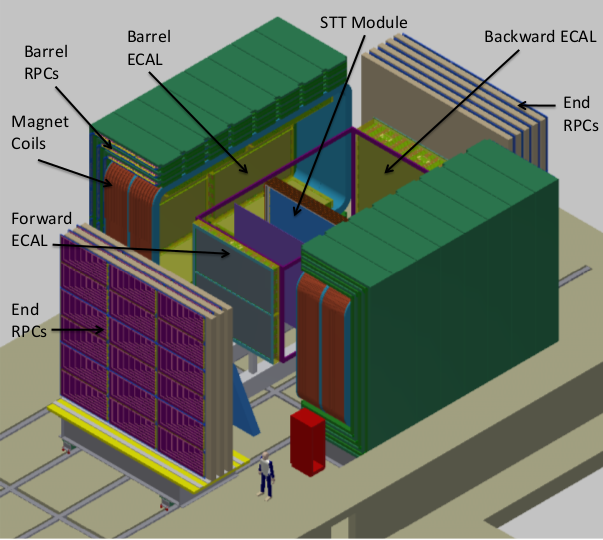
\includegraphics[width=0.50\textwidth, keepaspectratio=true]{figs/nearDetector.png}
\end{figure}
\scriptsize
The scheme of the near detector is shown at the fig. \ref{fig:nearDetector}. The detector will consist of central Straw-Tube Tracker (STT) modules, electromagnetic calorimeter (ECAL), magnet coils of 0.4T and muon identification system consisting of Resistive Plate Chamber (RPC) modules. The neutrinos would come from the bottom left corner of the picture, to the End RPCs.\\
\end{frame}

\begin{frame}\frametitle{LBNF. Near Detector Physics}
\scriptsize
\tiny
\begin{itemize}
  \item absolute flux measurement
  \item relative neutrino and antineutrino flux measurements
  \item flavor content of the neutrino source
  \item determination of the $E_\nu$-scale of neutrinos versus antineutrinos
  \item event-by-event measurements of NC interactions
  \item measurement of $\pi^0$, $\pi^\pm$, $K^\pm$, p, $K^0_S$ and $\Lambda$ in the NC and CC
%  \item "quasi-elastic and resonance measurements"
  \item nucleon structure, parton distribution functions and QCD studies
%  \item neutrino-argon interactions and nuclear effects
  \item precision measurements of electroweak physics
%  \item isospin physics and the Adler sum rule
%  \item measurement of the nuclean strangeness content
\end{itemize}

More specifically, the list of the physics measurements related to the neutrino oscillations to be performed by the Near Detector includes:
\begin{itemize}
  \item fluxes of $\nu_\mu$, $\bar{\nu_\mu}$, $\nu_e$ and $\bar{\nu_e}$. To distinguish between flavors, the measurement should rely on charged current interaction (fig. \ref{fig:MuonAndNeutronDecays}, middle and right) and measure the products of these interactions $\mu^-$, $\mu^+$, $e^-$, and $e^+$. (While the beam production system has the highest probability to produce muon neutrinos, the production of certain number electron neutrinos is also possible, for example, from charged kaon decays)
  \item $\nu_e$-$\bar{\nu_e}$ assymetries. For that, it's important not only distinguish between $\mu^\pm$ and $e^\pm$ but also between $e^-$ and $e^+$.
  \item the absolute $\nu_\mu$ and $\bar{\nu_\mu}$ fluxes need to be measured with $\simeq{3\%}$ precision in the neutrino energy range 0.5-8 GeV
  \item cross section of NC versus CC processes as a function of hadronic energy. NC is one of major backrounds which contribute to neutrino oscillation measurement
  \item yields of $\pi_0$ and photons. These particles are the most significant background to $\nu_e$ and $\bar{\nu_e}$ contamination
  \item fractions of the $\pi^\pm$ into the CC and the NC hadronic jets.    
\end{itemize} 
\end{frame}

\begin{frame}\frametitle{LBNF. SURF (Far Detector Site)}
\begin{figure}
\label{fig:farDetector_SURF1}
\centering
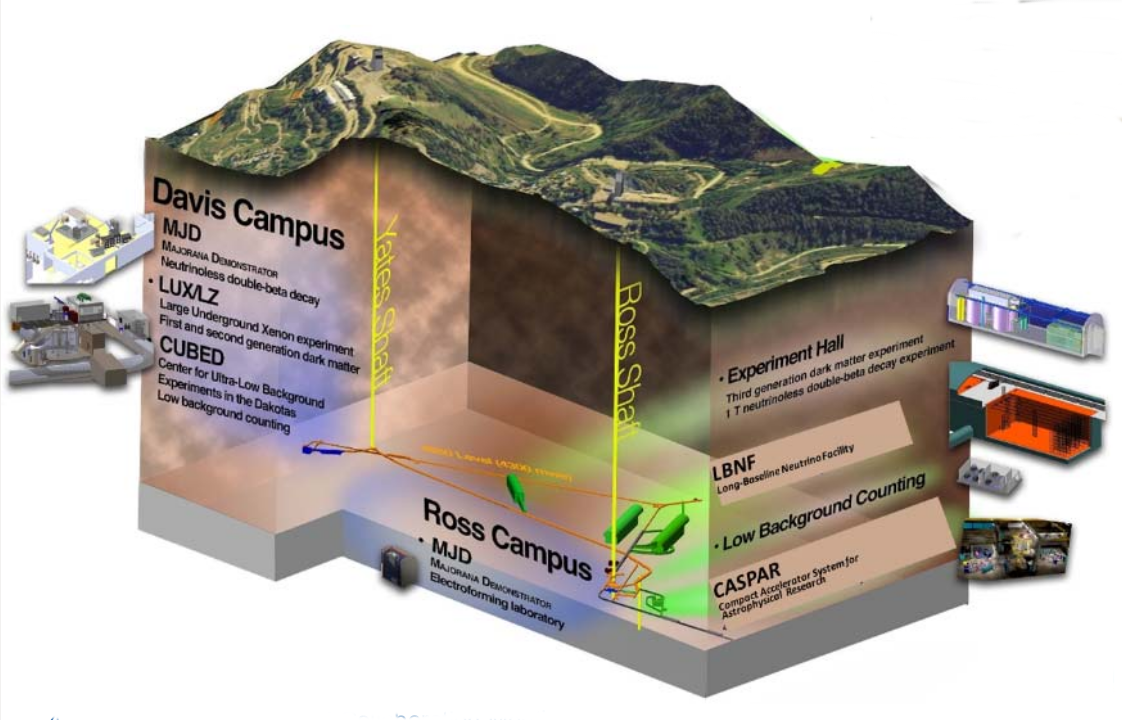
\includegraphics[width=0.98\textwidth, keepaspectratio=true]{figs/farDetector_SanfordUndergroundResearchFacility.png}
\end{figure}
\end{frame}

\begin{frame}\frametitle{LBNF. SURF (Far Detector Site)}
\begin{figure}
\label{fig:farDetector_SURF2}
\centering
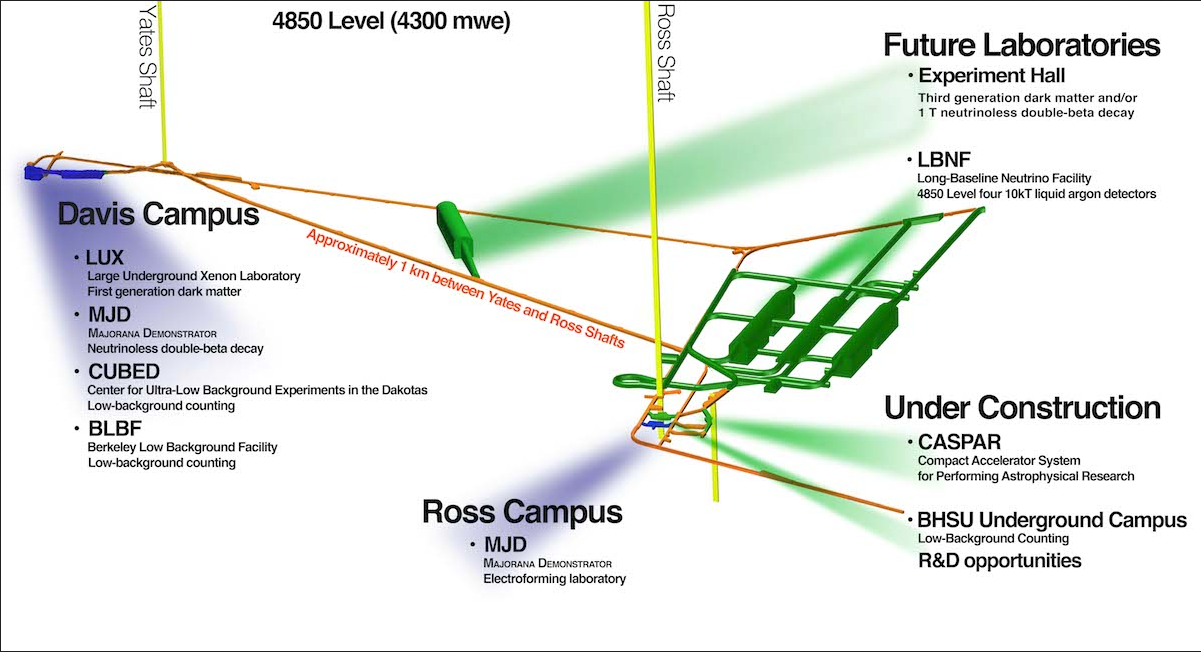
\includegraphics[width=0.98\textwidth, keepaspectratio=true]{figs/farDetector_wholeLab.png}
\end{figure}
\scriptsize
4 modules (15m x 12m x 58m, 10,000 tonnes of liquid argon each) placed into 4 caverns 1500 m underground. 5th cavern between two pairs - cryogenic equipment\\
\end{frame}

\begin{frame}\frametitle{LBNF. Far Detector. Liquid Argon Time Projection Chamber}
\begin{figure}
\label{fig:farDetector_TPC}
\centering
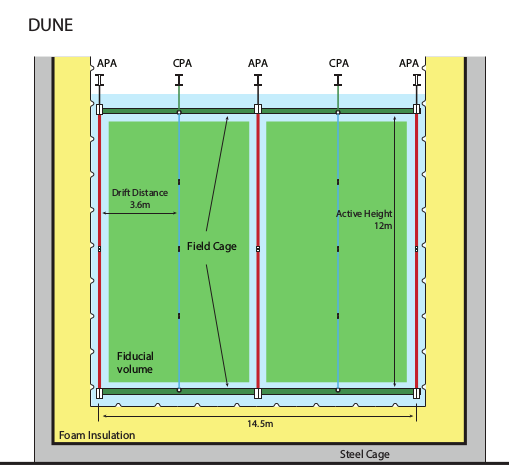
\includegraphics[width=0.75\textwidth, keepaspectratio=true]{figs/farDetector_TPC.png}
\end{figure}
\end{frame}

\begin{frame}\frametitle{LBNF Compared to the Other Experiments}
\tiny
  \begin{tabular}{|c|c|c|c|c|c|}
              & KEK (K2K) & NuMI & CNGS & T2K & LBNF (DUNE)\\ \hline
     location & Japan  & Illinois - & Switzerland - & Japan & Illinois - \\ 
              &        & Minnesota & Italy &  & South Dakota\\ \hline
     accelerator & KEK PS  & FNAL & CERN's SPS & J-PARC & FNAL\\ \hline
     time of oper. & 1999-2004  & 2005-2012 & 2006-2012 & 2010- & future \\ \hline 
     beam power  &  5 kW  & 300-350 kW  & 300 kW & 750 kW & 2000 kW\\ \hline 
     $E_p$  & 12 GeV & 120 GeV & 400 GeV & 30 GeV & 60-120 GeV\\ \hline 
     baseline  & 250 km & 735 km & 730 km & 295 km & 1300 km\\ \hline 
%                & KEK (K2K)   & NuMI                & CNGS                & T2K         & LBNF (DUNE)\\ \hline
     near        & (water ChD) & MINOS               & (muon               & ND280       & DUNE (FGD)\\  
     detector(s) & (FGD)       & (track. and scint.) & detector)           & INGRID      & \\ \hline 
     ND mass     & 1 kt (ChD)  & 0.98 kt             &                     &             & \\ \hline 
     far         & SuperK      & MINOS               & ICARUS (LAr)        & SuperK      & DUNE (LAr)\\  
     detector(s) & (water ChD) & track. and scint.   & OPERA (FGD)        & (water ChD) & \\ \hline 
     FD mass     & 50 kt       & 5.4 kt              & 0.76 kt (ICARUS)   & 50 kt       & 40 kt\\ 
                 &             &                     & 1.25 kt (OPERA)    &             & \\ \hline 
 \end{tabular}
\end{frame}

\begin{frame}\frametitle{LBNF. Status}
\scriptsize
\begin{itemize}
  \item Experiment is under development
  \item Conceptual Design Report (CDR) drafts are partially available
  \item First collaboration meeting took place on April 16th-18th, 2015
  \item Fermilab accelerator is available 
  \item Cavern for the near detector to be excavated
  \item Caverns for the far detector exist (former Homestake mine)
  \item far detector installation planned on 2021-2022
\end{itemize}
\end{frame}
